\pdfminorversion=4
\documentclass[aspectratio=169]{beamer}

\mode<presentation>
{
  \usetheme{default}
  \usecolortheme{default}
  \usefonttheme{default}
  \setbeamertemplate{navigation symbols}{}
  \setbeamertemplate{caption}[numbered]
  \setbeamertemplate{footline}[frame number]  % or "page number"
  \setbeamercolor{frametitle}{fg=white}
  \setbeamercolor{footline}{fg=black}
} 

\usepackage[english]{babel}
\usepackage[utf8x]{inputenc}
\usepackage{tikz}
\usepackage{courier}
\usepackage{array}
\usepackage{bold-extra}
\usepackage{minted}
\usepackage[thicklines]{cancel}
\usepackage{fancyvrb}

\xdefinecolor{dianablue}{rgb}{0.18,0.24,0.31}
\xdefinecolor{darkblue}{rgb}{0.1,0.1,0.7}
\xdefinecolor{darkgreen}{rgb}{0,0.5,0}
\xdefinecolor{darkgrey}{rgb}{0.35,0.35,0.35}
\xdefinecolor{darkorange}{rgb}{0.8,0.5,0}
\xdefinecolor{darkred}{rgb}{0.7,0,0}
\definecolor{darkgreen}{rgb}{0,0.6,0}
\definecolor{mauve}{rgb}{0.58,0,0.82}

\title[2022-03-21-reload-stats-of-physicists]{Metrics of computing trends in NHEP}
\author{Jim Pivarski}
\institute{Princeton University -- IRIS-HEP}
\date{March 21, 2022}

\usetikzlibrary{shapes.callouts}

\begin{document}

\logo{\pgfputat{\pgfxy(0.11, 7.4)}{\pgfbox[right,base]{\tikz{\filldraw[fill=dianablue, draw=none] (0 cm, 0 cm) rectangle (50 cm, 1 cm);}\mbox{\hspace{-8 cm}
\includegraphics[height=1 cm]{princeton-logo-long.png}\hspace{0.1 cm}\raisebox{0.1 cm}{
\includegraphics[height=0.8 cm]{iris-hep-logo-long.png}}\hspace{0.1 cm}}}}}

\begin{frame}
  \titlepage
\end{frame}

\logo{\pgfputat{\pgfxy(0.11, 7.4)}{\pgfbox[right,base]{\tikz{\filldraw[fill=dianablue, draw=none] (0 cm, 0 cm) rectangle (50 cm, 1 cm);}\mbox{\hspace{-8 cm}
\includegraphics[height=1 cm]{princeton-logo.png}\hspace{0.1 cm}\raisebox{0.1 cm}{
\includegraphics[height=0.8 cm]{iris-hep-logo.png}}\hspace{0.1 cm}}}}}

% Uncomment these lines for an automatically generated outline.
%\begin{frame}{Outline}
%  \tableofcontents
%\end{frame}

% START START START START START START START START START START START START START

\begin{frame}{\mbox{ }}
\large
\vspace{0.5 cm}
\begin{columns}
\column{0.7\linewidth}
This is a talk about measuring {\it physicists}: what they talk about and what they do for computing.

\vspace{0.25 cm}
\uncover<2->{Measuring people, such as advertising click-throughs, seemed odd to me when I first went from physics to data science, since the events are {\it not} independent and it would be hard to quantify errors.}

\vspace{0.25 cm}
\uncover<3->{However, it can be a meaningful thing to do, taking all the caveats seriously, and certainly better than {\it guessing} or {\it assuming} we understand the community.}

\vspace{0.25 cm}
\uncover<4->{Inspiration: read Sharon Traweek's anthropological study of physicists at SLAC and KEK in the 1970's. Physicists can be data points!}

\column{0.3\linewidth}
\uncover<4->{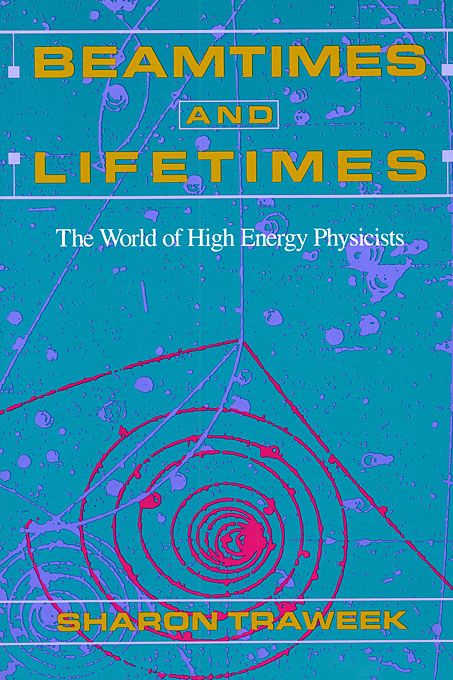
\includegraphics[width=\linewidth]{traweek-beamtimes-and-lifetimes.jpg}}
\end{columns}
\end{frame}

\begin{frame}{User needs are very different from my expectations, 5 years ago}
\vspace{0.25 cm}
\begin{columns}
\column{1.12\linewidth}
\only<1>{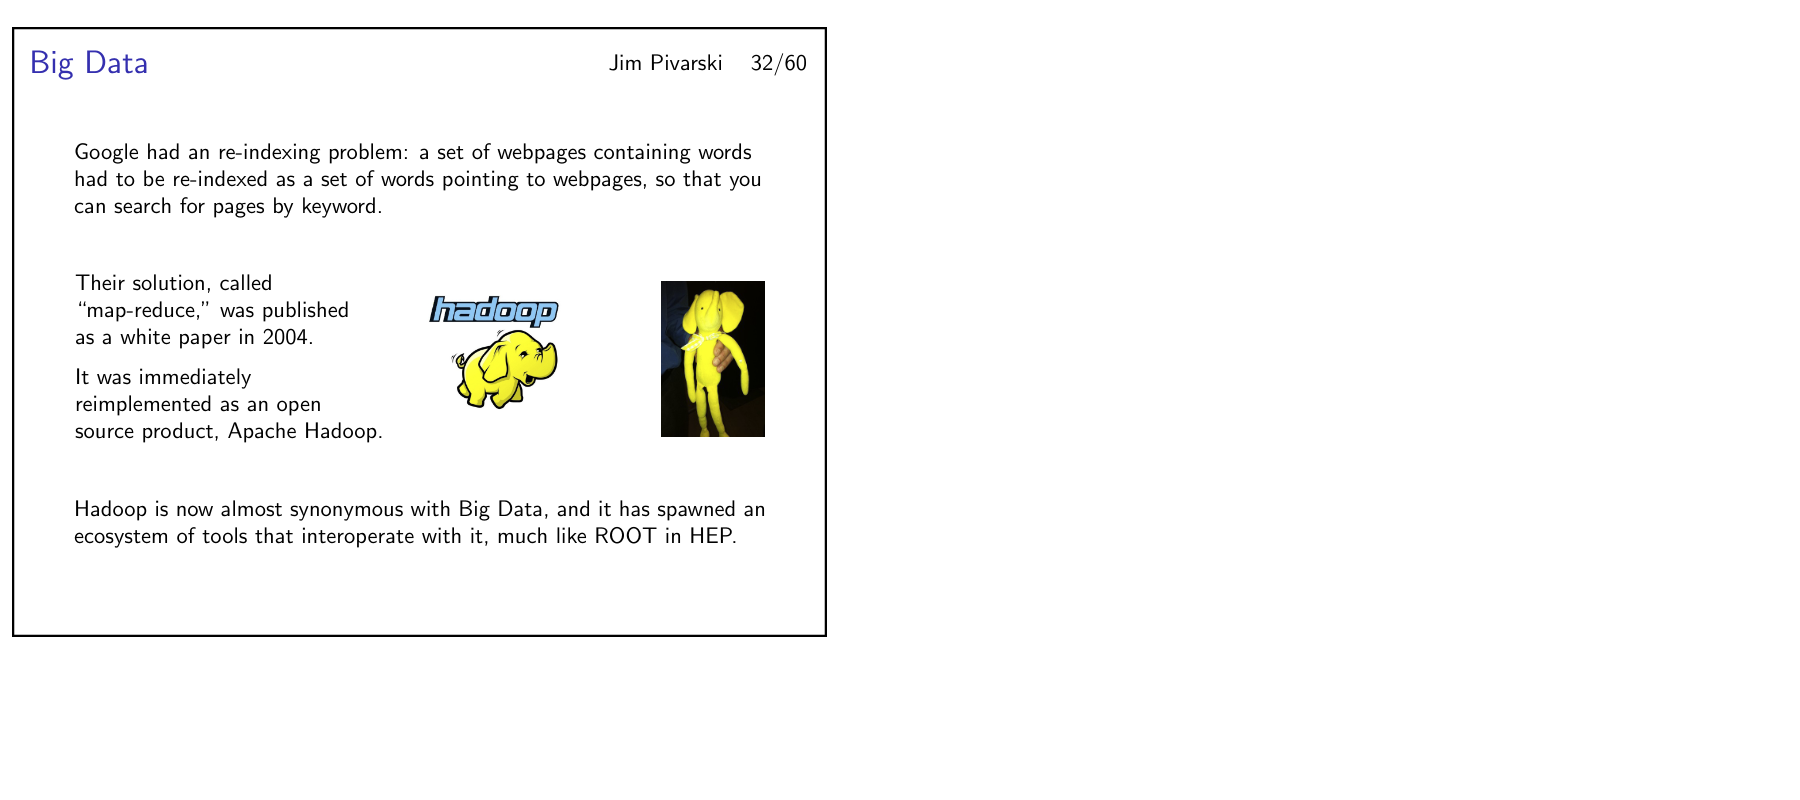
\includegraphics[width=\linewidth]{evolving-views-1.png}}\only<2>{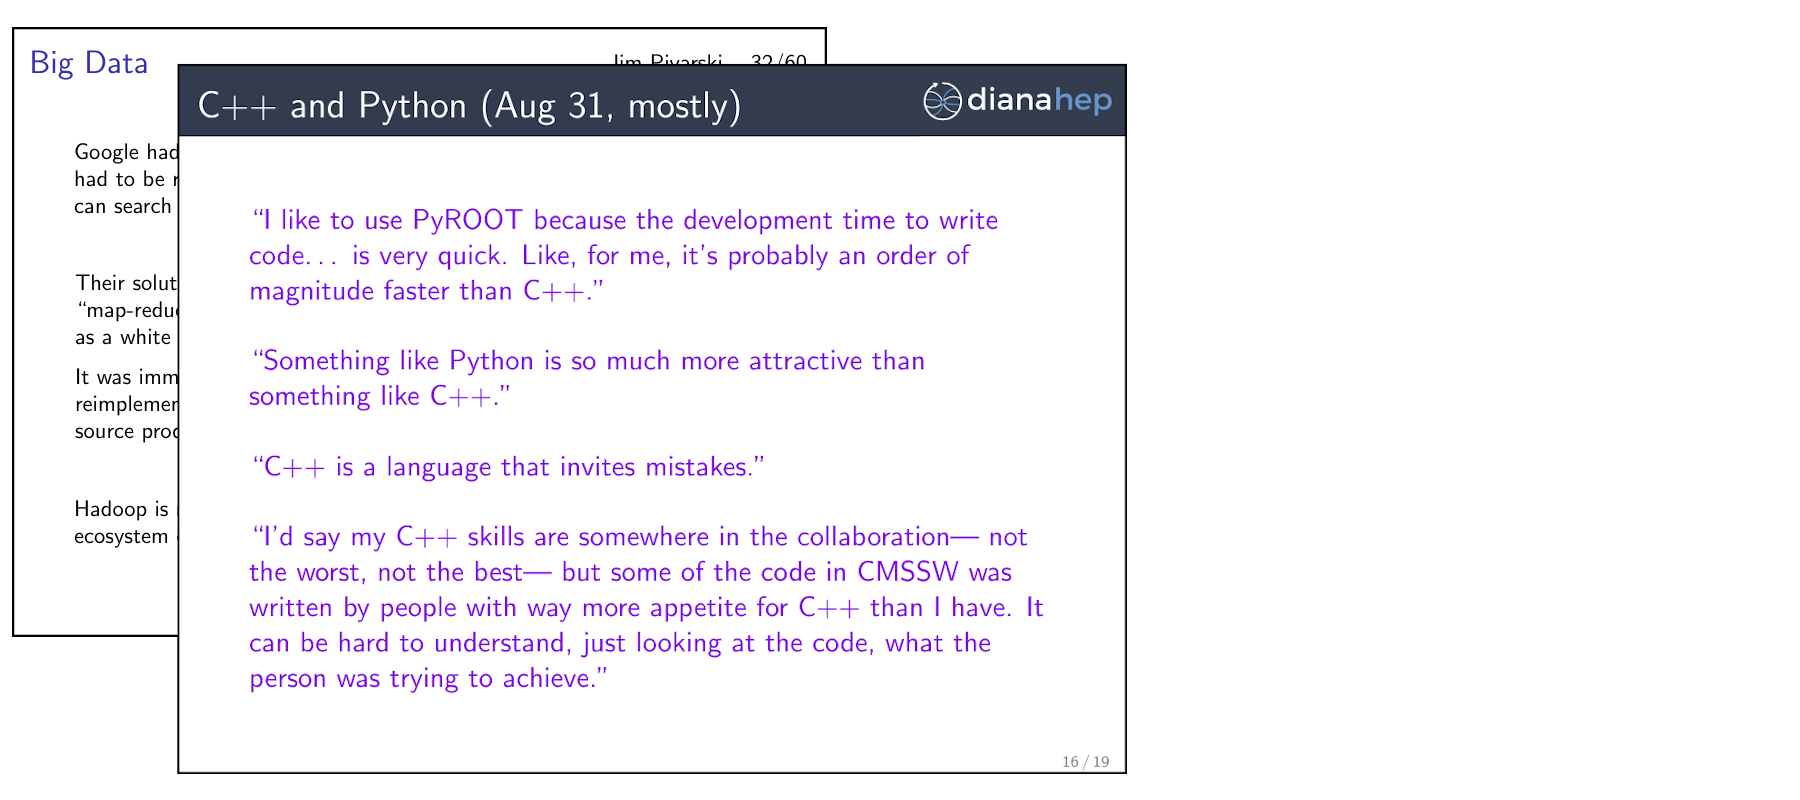
\includegraphics[width=\linewidth]{evolving-views-2.png}}\only<3>{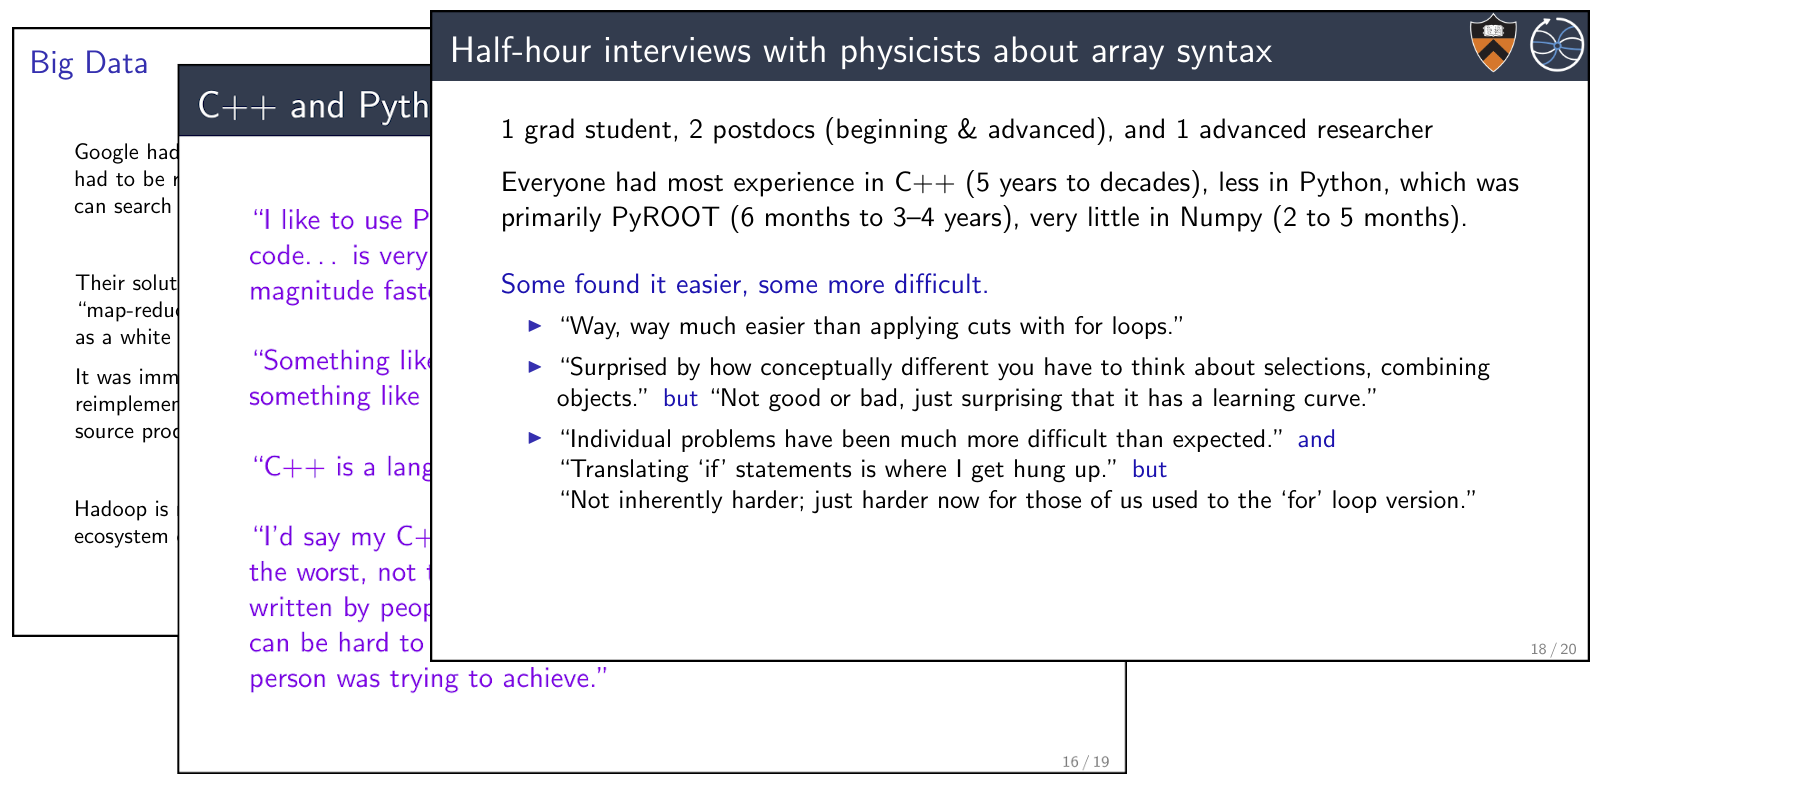
\includegraphics[width=\linewidth]{evolving-views-3.png}}\only<4>{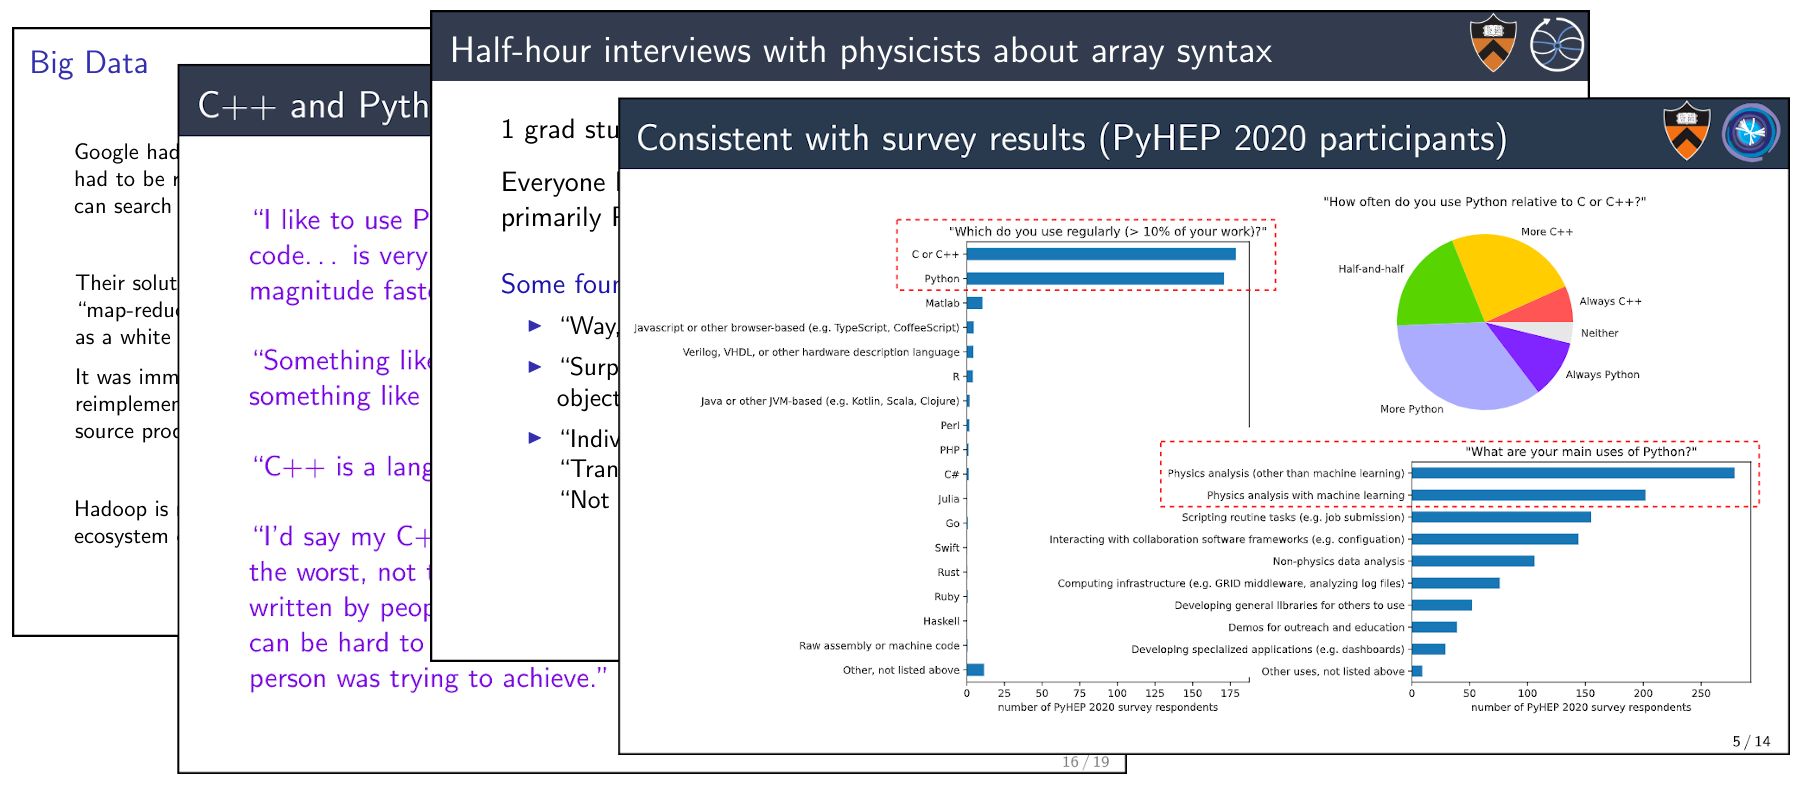
\includegraphics[width=\linewidth]{evolving-views-4.png}}
\end{columns}

\vspace{0.1 cm}
\uncover<2->{\Large\hfill Sought user input in focus groups, interviews, and surveys.}
\end{frame}

\begin{frame}{Ways to study humans}
\vspace{0.1 cm}
\textcolor{gray}{\scriptsize (Important note: I am not an expert. This is what I learned from college friends who went into social sciences.)}

\large
\vspace{0.1 cm}
\begin{itemize}\setlength{\itemsep}{0.25 cm}
\item \textcolor{darkblue}{Qualitative:}

\vspace{0.05 cm}
\begin{itemize}\large\setlength{\itemsep}{0.15 cm}
\item \textcolor{darkblue}{Focus groups:} \normalsize most open to unexpected ideas. Want to keep the group size and mix such that participants are willing to speak up. Goal is to discover new {\it dimensions} of the vector space, not just points within it. \large

\item \textcolor{darkblue}{One-on-one interviews:} \normalsize can go for depth, rather than breadth. Lacks the multiplying effect of responding to differing opinions. \large

\item \textcolor{darkblue}{History/documents:} \normalsize observational, rather than experimental, but this method can reach further into the past. \large
\end{itemize}

\item \textcolor{darkblue}{Quantitative:}

\vspace{0.05 cm}
\begin{itemize}\large\setlength{\itemsep}{0.15 cm}
\item \textcolor{darkblue}{Surveys:} \normalsize can have large datasets, at the cost of losing flexibility/openness to new ideas. Now you {\it are} filling in a vector space. \large

\item \textcolor{darkblue}{Proxy metrics:} \normalsize can measure what people {\it do}, rather than what they {\it say}. \large
\end{itemize}

\end{itemize}
\end{frame}

\begin{frame}{Proxy metrics: high statistics, cautious interpretation}
\vspace{0.25 cm}
\mbox{\hspace{0.75 cm}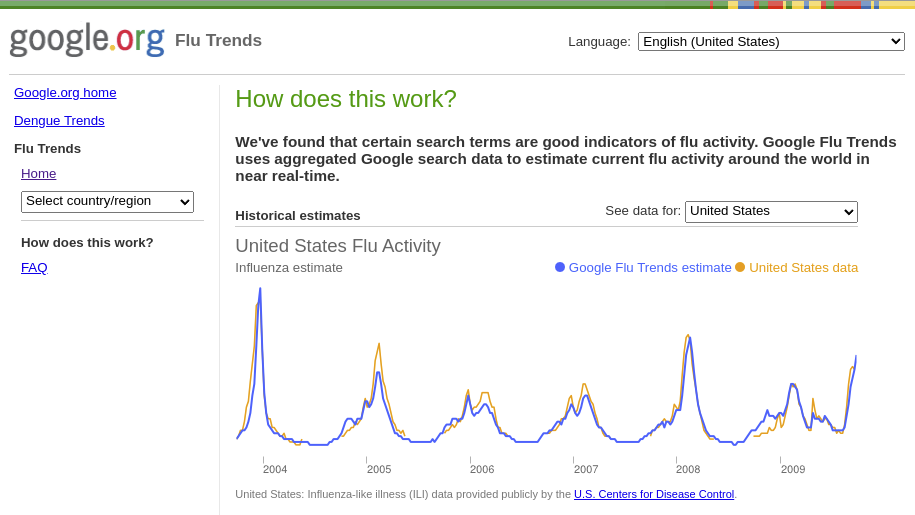
\includegraphics[width=\linewidth]{google-flu-trends.png}}

\vspace{-3.35 cm}
\hspace{-0.25 cm}\begin{minipage}{0.3\linewidth}
{\bf Google Flu Trends}

{\bf (2008--2015)}

\small
\vspace{0.25 cm}
Count searches for

things like ``fever,'' ``cough,''

interpret as flu activity.

\vspace{0.25 cm}
(This was controversial.)
\end{minipage}
\vspace{3.35 cm}
\end{frame}

\begin{frame}{}




\end{frame}



\end{document}
